\documentclass[11pt,a4paper]{article}
\usepackage[a4paper,hmargin=1in,vmargin=1in]{geometry}
\usepackage{pgfplots}
\pgfplotsset{compat=1.17}

\usepackage[czech]{babel}
\usepackage[utf8]{inputenc}
\usepackage[T1]{fontenc}

\usepackage[nodayofweek]{datetime}
\newdate{date}{17}{6}{2023}

\usepackage{stddoc}
\usepackage{lipsum}
\usepackage{subcaption}
% \usepackage[square,numbers]{natbib}
% \usepackage[nottoc]{tocbibind}

\newcommand{\plus}{{\texttt{+}}}
\renewcommand{\Re}{\operatorname{Re}}
\renewcommand{\Im}{\operatorname{Im}}
\newcommand{\fourier}[3]{\mathcal{F}_{#1}\!\left[#2\right]\!\left(#3\right)}
\newcommand{\ifourier}[3]{\mathcal{F}^{-1}_{#1}\!\left[#2\right]\!\left(#3\right)}
\newcommand{\Ohm}{\mathrm{\Omega}}
\newcommand{\kOhm}{\mathrm{k\Omega}}
\newcommand{\dB}{\mathrm{dB}}
\newcommand{\dBm}{\mathrm{dBm}}
\newcommand{\MHz}{\mathrm{MHz}}
\newcommand{\GHz}{\mathrm{GHz}}
\newcommand{\kHz}{\mathrm{kHz}}
\newcommand{\mm}{\mathrm{mm}}
\newcommand{\mum}{\mathrm{\mu m}}


\begin{document}

\pagenumbering{arabic}

% Header
\begin{center}
    {\LARGE\textbf{Laboratorní úloha č. 13}}\\[3mm]
    \begin{minipage}{0.4\textwidth}
        \begin{flushleft}
            \textsc{\displaydate{date}}
        \end{flushleft}
    \end{minipage}
    ~
    \begin{minipage}{0.4\textwidth}
        \begin{flushright}
            \textsc{Martin Šimák}
        \end{flushright}
    \end{minipage}
    \noindent\rule{14.5cm}{0.4pt}
\end{center}

\paragraph*{Měření S-parametrů tranzistoru} Laboratorní úloha ukazuje využití vektorového měření pro určování parametrů tranzistoru v SMD pouzdru s referenční rovinou uprostřed pouzdra.

\subsection*{Úkoly měření}
\begin{enumerate}
    \item Změřte S-parametry tranzistoru Avago ATF 36077 v pouzdru o průměru 5.28~mm namontovaného do mikropáskového vedení ve frekvenčním pásmu 4~GHz až 20~GHz při různých způsobech montáže: elektrody source \uv{podloženy} mikropáskovým vedením délky 0~mm, 0.5~mm a 1.6~mm.
    \item Referenční rovinu změřených S-parametrů přetransformujte na okraje pouzdra.
\end{enumerate}

\subsection*{Použité přístroje a komponenty}
\begin{itemize}
    \item Agilent PNA E8364A (45~MHz až 50~GHz)
    \item Měřicí držák délky 50~mm s SMA konektory
\end{itemize}

\subsection*{Popis měření}
Měření provádíme na mikrovlnném držáku pro planární vedení na $50\Ohm$ mikropáskovém vedení na substrátu Rogers CuClad 233, $h = 0.508\ \mm$, $\epsilon_r = 2.33$, $t = 17\ \mum$ a k měření využíváme vektorového analyzátoru obvodů Agilent PNA E8364A. Pracovní bod tranzistoru volíme $(1.5\ \mathrm{V},10\ \mathrm{mA})$. Kalibrujeme přímo na držáku metodou OSMT, k níž používáme posuvnou mikropáskovou bezodrazovou koncovku a mikropáskové přípravky z kalibry. Držák kalibrujeme do středu, tj. referenční rovina měření bude uprostřed měřených tranzistorů. Postupně měříme S-parametry tranzistorů ve všech konfiguracích montáže. Výsledné průběhy exportujeme a zpracováváme v AWR.

Pro zpracování dat postupujeme tak, že nejprve porovnáme čistá naměřená data jako blok S-parametrů s daty dodanými výrobcem, které jsou dostupné pro simulace v knihovnách softwaru AWR. Jak je vidět z obrázku~\ref{fig:0mm-center}, data od výrobce jsou zřejmě též měřena s referenční rovinou uprostřed pouzdra, jelikož sledují velice podobný průběh jako data experimentální.
\begin{figure}[!ht]
    \centering
\begin{subfigure}{0.45\textwidth}
    \centering
    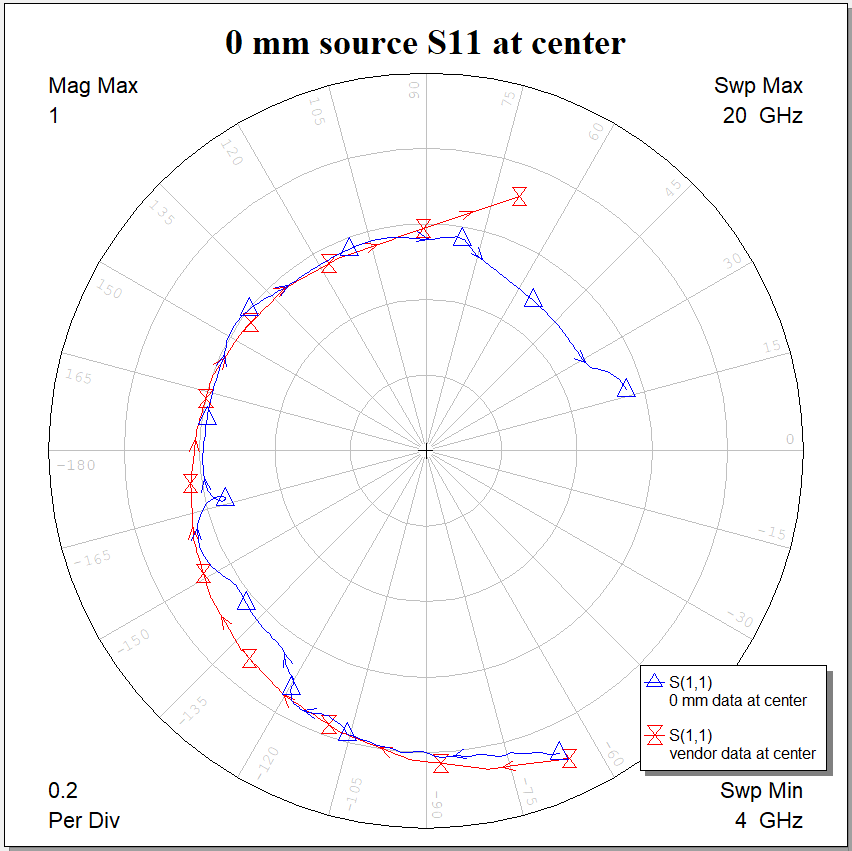
\includegraphics[width=\textwidth]{src/0mm-S11-center.png}
    \caption{Odraz $S_{11}$}
\end{subfigure}
\begin{subfigure}{0.45\textwidth}
    \centering
    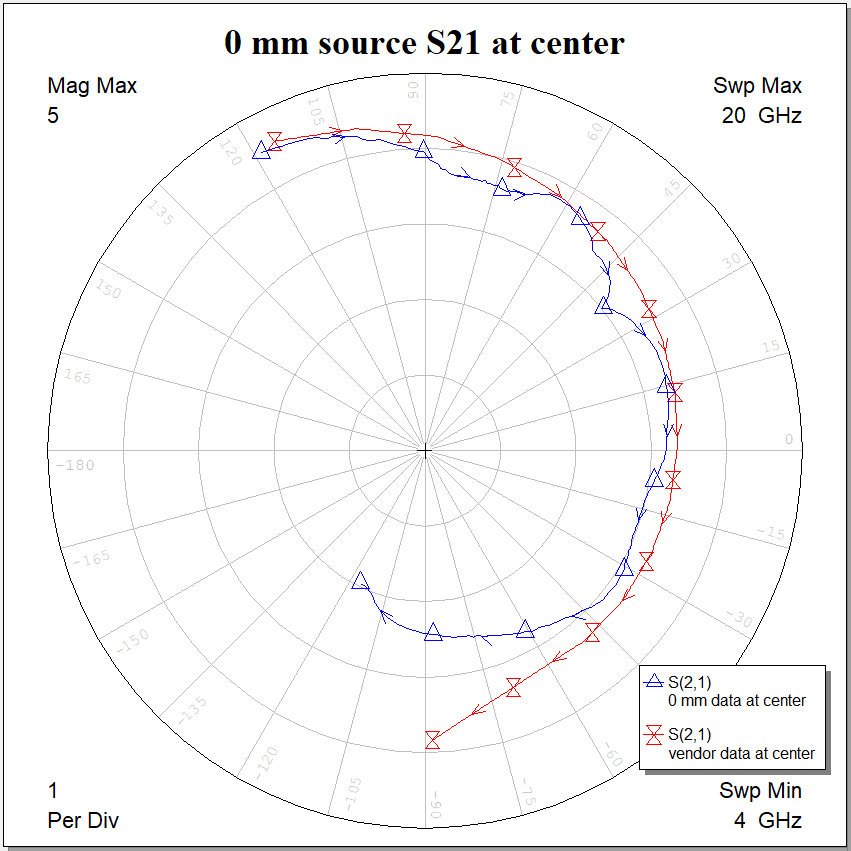
\includegraphics[width=\textwidth]{src/0mm-S21-center.png}
    \caption{Přenos $S_{21}$}
\end{subfigure}
\caption{\label{fig:0mm-center}Porovnání naměřených dat s podložením 0 mm s daty od výrobce}
\end{figure}

Dále proto k datům experimentálním i těch od výrobce v AWR vložíme před a za referenční rovinu $50\Ohm$ mikropáskové vedení s délkou odpovídající poloměru pouzdra tranzitoru. Simulací těchto obvodů určíme výsledné S-parametry obvodu v požadovaných referenčních rovinách na okrajích pouzdra. Výsledky je možně opět porovnat na obrázku~\ref{fig:0mm}.
\begin{figure}[!ht]
    \centering
\begin{subfigure}{0.45\textwidth}
    \centering
    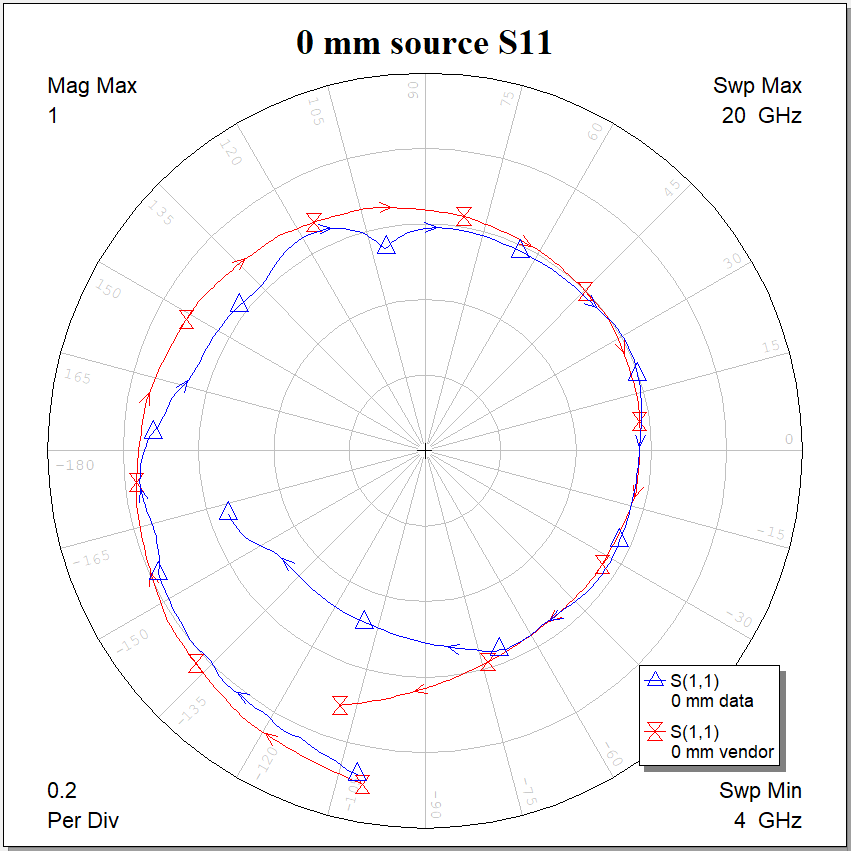
\includegraphics[width=\textwidth]{src/0mm-S11.png}
    \caption{Odraz $S_{11}$}
\end{subfigure}
\begin{subfigure}{0.45\textwidth}
    \centering
    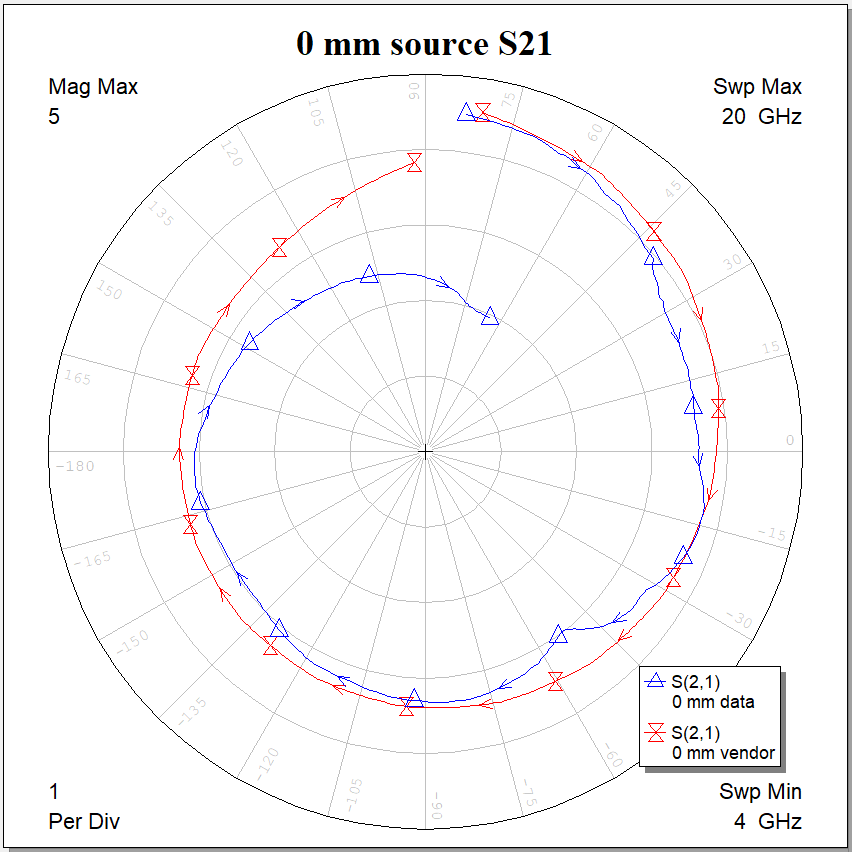
\includegraphics[width=\textwidth]{src/0mm-S21.png}
    \caption{Přenos $S_{21}$}
\end{subfigure}
\caption{\label{fig:0mm}Porovnání dat s podložením 0 mm na okrajích pouzdra}
\end{figure}

Zbylá data jsou měřena s podložením source elektrod mikropáskovým vedením. Tato data tedy vykreslujeme v porovnání s S-parametry dodanými výrobcem v AWR pomocí obvodu s explicitně definovanou zemí. Mezi blok S-parametrů představující tranzitor a explicitní zemní elektrodu vložíme onen úsek příslušné délky. Výsledky porovnání jsou obsaženy v grafech na obrázku~\ref{fig:0m5m} pro podložení délky 0.5~mm a na obrázku~\ref{fig:1m6m} pro podložení 1.6~mm.
\begin{figure}[!ht]
    \centering
\begin{subfigure}{0.45\textwidth}
    \centering
    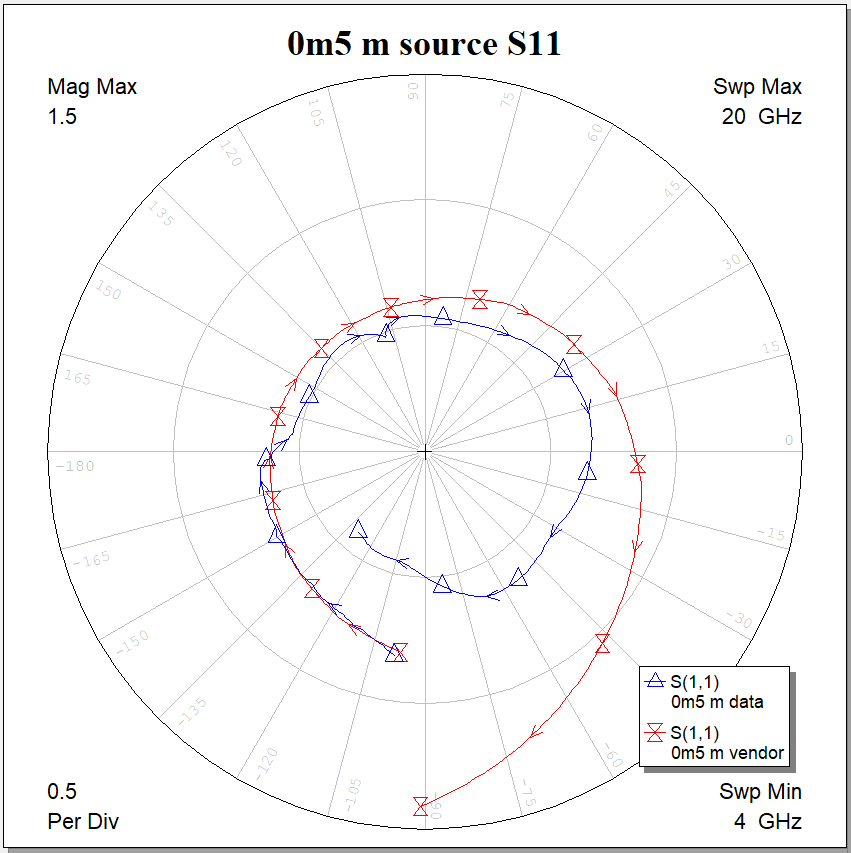
\includegraphics[width=\textwidth]{src/0m5m-S11.png}
    \caption{Odraz $S_{11}$}
\end{subfigure}
\begin{subfigure}{0.45\textwidth}
    \centering
    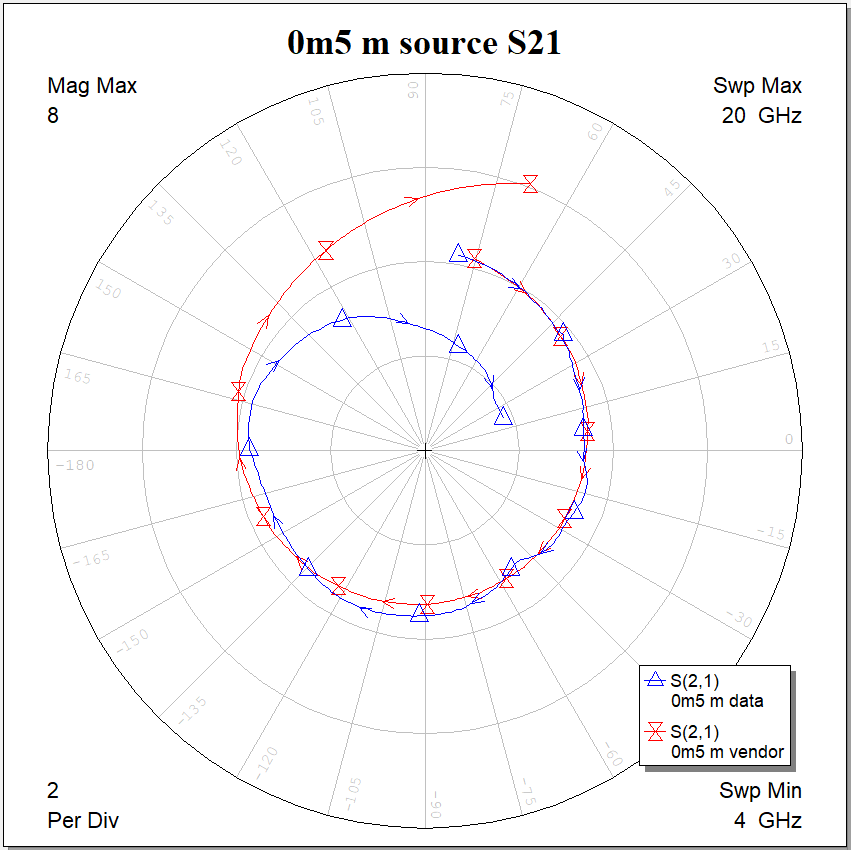
\includegraphics[width=\textwidth]{src/0m5m-S21.png}
    \caption{Přenos $S_{21}$}
\end{subfigure}
\caption{\label{fig:0m5m}Porovnání dat s podložením 0.5 mm na okrajích pouzdra}
\end{figure}
\begin{figure}[!ht]
    \centering
\begin{subfigure}{0.45\textwidth}
    \centering
    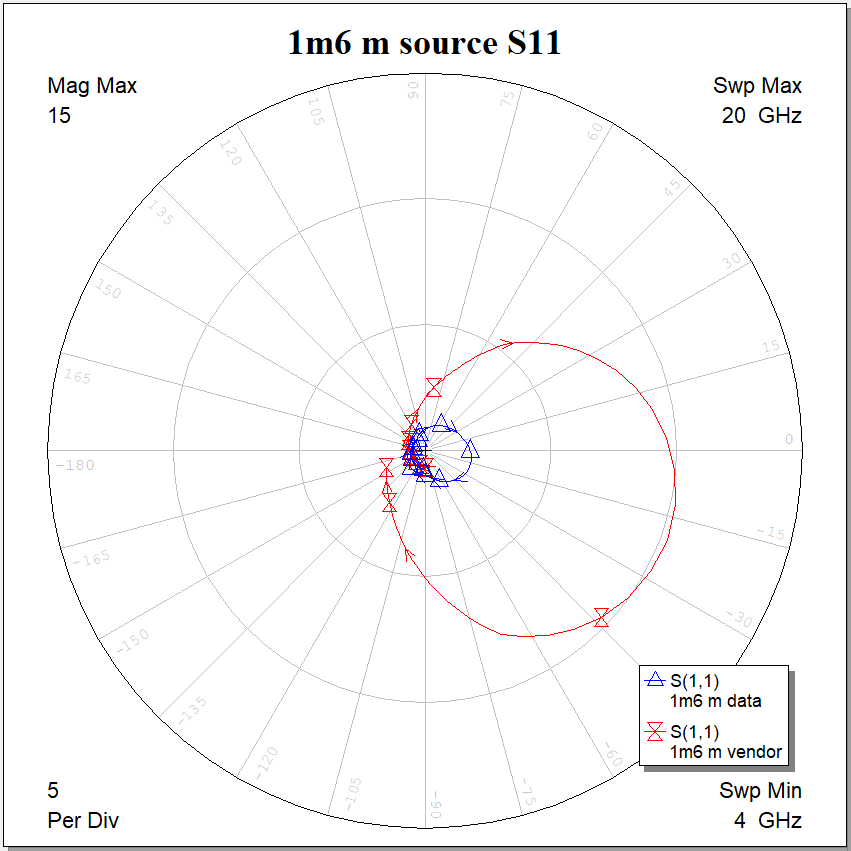
\includegraphics[width=\textwidth]{src/1m6m-S11.png}
    \caption{Odraz $S_{11}$}
\end{subfigure}
\begin{subfigure}{0.45\textwidth}
    \centering
    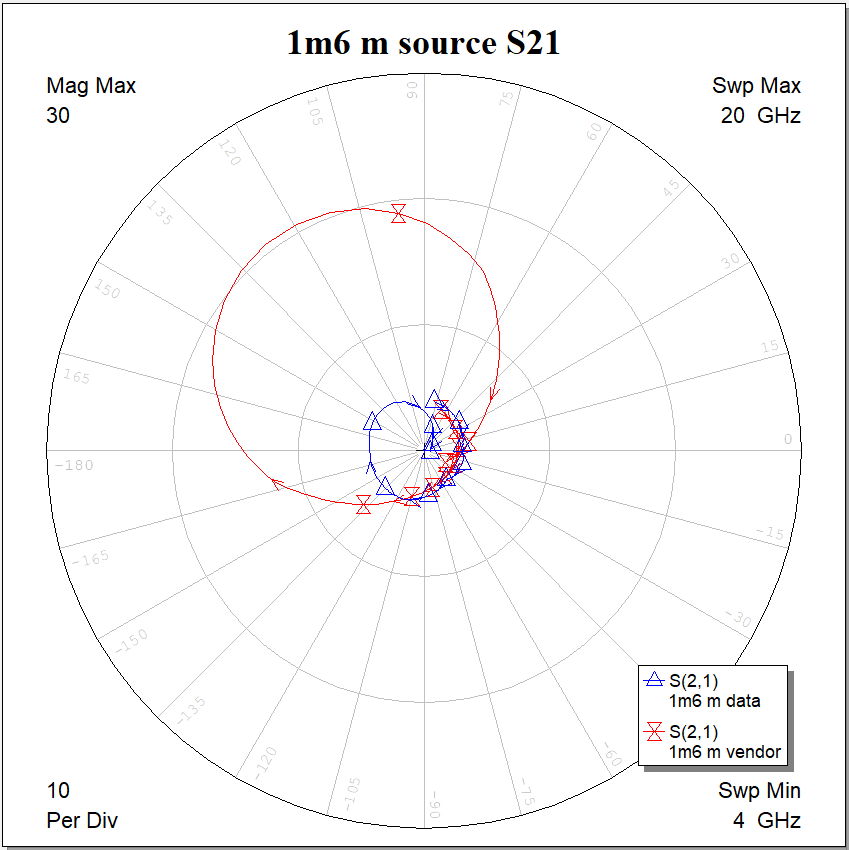
\includegraphics[width=\textwidth]{src/1m6m-S21.png}
    \caption{Přenos $S_{21}$}
\end{subfigure}
\caption{\label{fig:1m6m}Porovnání dat s podložením 1.6 mm na okrajích pouzdra}
\end{figure}

V grafech odrazu od tranzistoru s podloženými source elektrody si můžeme povšimnout nestabilních tendencí. To koreluje se zkušeností z návrhu mikrovlnných oscilátorů, kde jsme právě přidávali takové zpětnovazební elektrody, abychom dosáhli nestability obvodu. Bohužel také můžeme pozorovat již velice značné nesrovnalosti s daty od výrobce, zejména pro delší vedení na source elektrodách.

\subsection*{Závěr}
V rámci laboratorní úlohy jsme se seznámili s využitím vektorového měření pro určování parametrů tranzistoru v SMD pouzdru s referenční rovinou uprostřed pouzdra. Během zpracování jsme si tak vyzkoušeli běžně nutnou operaci transformace referenční roviny měření na okraj pouzdra. Dále jsme pozorovali vliv podložení source elektrod kusem mikropáskového vedení a i tyto případy jsme simulovali pro S-parametry od výrobce. Měření proběhlo bez větších potíží s největší deviací dat v případě podložení elektrod delším kusem mikropáskového vedení. V tomto případě je nesrovnalost s daty dodanými výrobcem již značná a pravděpodobně způsobena nepřesným měřením či horší opakovatelností měření v držáku.

\end{document}
